\documentclass[12pt,a4paper]{article}

\usepackage[utf8]{inputenc}
\usepackage[T1]{fontenc}
\usepackage{lmodern}
\usepackage[brazilian]{babel}
\usepackage[a4paper,margin=2.5cm]{geometry}
\usepackage{graphicx}
\usepackage{booktabs}
\usepackage{tabularx}
\usepackage{array}
\usepackage{amsmath}
\usepackage{xcolor}
\usepackage{enumitem}
\usepackage{float}
\usepackage{caption}
\usepackage{fancyhdr}
\usepackage{listings}
\usepackage{microtype}
\usepackage[hidelinks]{hyperref}

\definecolor{wegblue}{HTML}{00579D}
\definecolor{codebg}{HTML}{F5F7FA}
\definecolor{codeframe}{HTML}{CBD3DE}

\hypersetup{pdftitle={PredictaMaq: Relatório Técnico},pdfauthor={Equipe 2}}
\captionsetup{font=small,labelfont=bf}
\setlist{itemsep=2pt,topsep=4pt}
\setlength{\parindent}{1.25cm}
\setlength{\parskip}{3pt}
\renewcommand{\arraystretch}{1.25}

\pagestyle{fancy}
\fancyhf{}
\fancyhead[L]{\small PredictaMaq --- Relatório Técnico}
\fancyhead[R]{\small Equipe 2}
\fancyfoot[C]{\small\thepage}
\renewcommand{\headrulewidth}{0.3pt}
\setlength{\headheight}{15pt}

\lstset{
  basicstyle=\ttfamily\footnotesize, backgroundcolor=\color{codebg}, frame=single, rulecolor=\color{codeframe},
  breaklines=true, columns=fullflexible, keepspaces=true, showstringspaces=false,
  literate={á}{{\'a}}1 {é}{{\'e}}1 {í}{{\'i}}1 {ó}{{\'o}}1 {ú}{{\'u}}1 {ã}{{\~a}}1 {õ}{{\~o}}1 {ç}{{\c c}}1 {â}{{\^a}}1 {ê}{{\^e}}1
}

\newcommand{\codigo}[1]{\texttt{\small #1}}
\newcommand{\fig}[3]{%
  \begin{figure}[H]\centering
  \includegraphics[width=#2\textwidth]{figuras/#1}
  \caption{#3}\label{fig:#1}
  \end{figure}}

\begin{document}

% ------------------------------------------------------------------ CAPA
\begin{titlepage}
\centering
\vspace*{1.5cm}
{\large Trabalho de Pesquisa e Aplicação Prática}\\[0.3cm]
{\large Engenharia e Design de Interfaces Analíticas na Indústria 4.0}\\[2.2cm]
{\Huge\bfseries\color{wegblue} PredictaMaq}\\[0.5cm]
{\Large Manutenção Preditiva e Telemetria de Maquinário Crítico\\(Prensas, Compressores e Tornos CNC)}\\[1.5cm]
{\large Relatório Técnico}\\[3cm]
\textbf{Equipe 2}\\[0.2cm]
\textit{[Inserir nomes dos integrantes]}\\[0.2cm]
\textit{[Inserir curso, turma e docente]}\\[2cm]
\today

\vfill
{\footnotesize Protótipo acadêmico com dados fictícios. A paleta azul é inspirada na identidade visual da WEG; o projeto não tem vínculo com a empresa.}
\end{titlepage}

\tableofcontents
\newpage

% ------------------------------------------------------------------ RESUMO
\section*{Resumo}
\addcontentsline{toc}{section}{Resumo}
Este relatório documenta o desenvolvimento do \emph{PredictaMaq}, uma aplicação web que simula o painel de um engenheiro de manutenção
e confiabilidade monitorando prensas hidráulicas, compressores de parafuso e tornos CNC por meio de telemetria de vibração, temperatura e
pressão. O sistema gera dados fictícios, armazena-os em arquivos CSV, transmite leituras em tempo real por WebSocket, calcula um índice de
saúde, detecta anomalias, estima a vida útil restante (RUL) e gerencia alertas e ordens de serviço. O \textbf{framework de código} utilizado é o
\textbf{Dash (Plotly)}, sobre Flask, conforme a stack recomendada para a Equipe 2 na proposta do trabalho. O relatório descreve a fundamentação
teórica, as decisões de arquitetura, o processo de desenvolvimento (incluindo um redesenho completo da interface após avaliação crítica), os testes,
as limitações do protótipo e o mapeamento às capacidades avaliadas na rubrica.

\medskip
\noindent\textbf{Palavras-chave:} manutenção preditiva; telemetria; visualização de dados; Dash; Plotly; WebSocket; usabilidade.

\newpage
% ------------------------------------------------------------------ 1
\section{Introdução}
\subsection{Contexto e objetivo}
A proposta de trabalho pede a construção de interfaces analíticas para o ambiente fabril da Indústria~4.0, unindo fundamentos de design visual,
desenvolvimento web, análise de dados e ferramentas de \emph{Business Intelligence}. Cada equipe recebeu um tema específico; o da Equipe~2 é
\textbf{Manutenção Preditiva e Telemetria de Maquinário Crítico (prensas/compressores)}. O enunciado detalha que o painel deve processar séries
temporais de vibração, temperatura e pressão e emitir alertas visuais imediatos em caso de desvio dos limites operacionais, tendo como público-alvo
\emph{engenheiros de manutenção e equipe de confiabilidade}.

O objetivo do projeto foi construir uma aplicação web operacional, com dados fictícios persistidos em CSV, que demonstrasse ao mesmo tempo o tema
específico (manutenção preditiva) e o tema geral exigido de todas as equipes: fundamentos de UX, frameworks de código, integração web e ferramentas de BI.

\subsection{Escopo}
\begin{itemize}
  \item Seis máquinas: duas prensas hidráulicas (PR-01, PR-02), dois compressores de parafuso (CP-01, CP-02) e dois tornos CNC (CNC-01, CNC-02).
  \item Três variáveis por máquina: vibração (mm/s), temperatura (\textdegree C) e pressão (bar).
  \item Histórico de 14 dias (leituras a cada 10 minutos) e telemetria ao vivo (uma leitura a cada 2 segundos).
  \item Análise: índice de saúde, anomalias, tendência e vida útil restante (RUL).
  \item Fluxo de manutenção: alerta $\rightarrow$ reconhecimento $\rightarrow$ ordem de serviço $\rightarrow$ conclusão.
\end{itemize}

% ------------------------------------------------------------------ 2
\section{Resposta direta: qual framework de código foi utilizado?}
\label{sec:framework}
O framework principal é o \textbf{Dash}, da Plotly (versão 4.4.1 no ambiente de desenvolvimento), escrito em \textbf{Python}. O Dash executa
sobre o servidor \textbf{Flask} e renderiza os gráficos com a biblioteca \textbf{Plotly} (Plotly.js no navegador). A escolha segue a stack
recomendada no quadro de equipes da proposta para o tema da Equipe~2: \emph{Python (Plotly/Dash) + WebSockets/Streaming + API de Sensores}.

\begin{table}[H]
\centering
\caption{Tecnologias utilizadas e seus papéis.}
\label{tab:stack}
\begin{tabularx}{\textwidth}{@{}l l X@{}}
\toprule
\textbf{Camada} & \textbf{Tecnologia} & \textbf{Papel no projeto}\\
\midrule
Framework de interface & Dash 4.4 (Plotly) & Layout, roteamento, callbacks reativos e componentes (\codigo{dcc}, \codigo{html}).\\
Gráficos & Plotly 7.1 (Plotly.js) & Séries temporais, projeção de tendência, barras, zonas de limite.\\
Servidor web & Flask 3.1 & Serve a aplicação Dash e as rotas REST (\codigo{/api/*}).\\
Tempo real & Flask-Sock 0.7 & Endpoint WebSocket \codigo{/ws} que envia cada leitura aos navegadores.\\
Dados e análise & pandas 3.0, NumPy 2.4 & Leitura de CSV, reamostragem, regressão, estatísticas robustas.\\
Persistência & Arquivos CSV & ``Banco'' de histórico, telemetria ao vivo, alertas e ordens de serviço.\\
Front-end próprio & HTML5, CSS3, JavaScript & Tema claro/escuro, layout responsivo e cliente WebSocket (\codigo{assets/}).\\
Qualidade (desenvolvimento) & pytest, Playwright & Testes unitários da análise e testes ponta a ponta no navegador.\\
\bottomrule
\end{tabularx}
\end{table}

Não foram utilizados D3.js, Chart.js, Streamlit nem ferramentas de BI de mercado (Power BI, Tableau) na implementação; esses itens aparecem
na comparação teórica da Seção~\ref{sec:fundamentacao}. As versões acima são as instaladas durante o desenvolvimento; o arquivo
\codigo{requirements.txt} fixa apenas versões mínimas.

% ------------------------------------------------------------------ 3
\section{Fundamentação teórica}
\label{sec:fundamentacao}
\begin{quote}\small
\textbf{Nota:} as referências citadas nesta seção e na bibliografia são pontos de partida levantados durante o projeto. Edição, ano e conteúdo
devem ser conferidos nas fontes originais antes da entrega final.
\end{quote}

\subsection{Fundamentos de UX para visualização de dados}
A proposta cita explicitamente as Leis da Gestalt, a hierarquia visual, o contraste, as paletas de cores acessíveis e a gestão da carga cognitiva.
Esses conceitos orientaram as decisões de interface:

\begin{description}[leftmargin=0.5cm,style=nextline]
  \item[Proximidade e região comum.] Elementos relacionados devem ficar próximos e, se possível, contidos numa mesma região. No projeto, cada máquina
  é um cartão; o espaço entre seções é maior que o espaço dentro delas.
  \item[Similaridade.] Elementos com a mesma função têm a mesma aparência. O estado de uma máquina é sempre exibido por um mesmo componente (``chip''),
  com a mesma lógica de cor e forma em todas as telas.
  \item[Continuidade e alinhamento.] A lista de máquinas usa colunas alinhadas, permitindo comparar valores por varredura vertical.
  \item[Figura-fundo.] Nos gráficos, a série ocupa o primeiro plano e as zonas de atenção e crítico aparecem como fundo translúcido.
  \item[Hierarquia visual.] Cada tela tem um elemento dominante (por exemplo, a frase de estado da planta ou os dias restantes até o limite crítico),
  seguido de informação secundária e, por último, detalhes.
  \item[Carga cognitiva e revelação progressiva.] Uma pergunta por tela, uma variável por gráfico, e detalhes técnicos escondidos em blocos recolhíveis.
  \item[Cor acessível.] O estado nunca depende só da cor: usa-se cor, forma (círculo, triângulo, quadrado) e texto. Os contrastes foram calculados
  (Seção~\ref{sec:cores}), seguindo os critérios de contraste da WCAG~2.x.
\end{description}

\subsection{Manutenção preditiva e monitoramento de condição}
A manutenção pode ser corretiva (após a falha), preventiva (por calendário) ou preditiva (baseada na condição real do ativo). O monitoramento de condição
mede grandezas como vibração, temperatura e pressão e as compara com zonas de severidade (normal, atenção, crítico). A estimativa de vida útil restante
(\emph{Remaining Useful Life}, RUL) projeta a evolução de um indicador de degradação até um limite de falha. Normas de referência na área incluem a
ISO~20816 (vibração em máquinas), a ISO~17359 (diretrizes de monitoramento de condição) e a ISO~13374 (processamento e apresentação de dados).
\textbf{Neste projeto, os limites numéricos são fictícios e didáticos}, não derivados de norma ou fabricante.

\subsection{Frameworks de código para visualização}
\begin{table}[H]
\centering
\caption{Comparativo de tecnologias de visualização considerado pela equipe.}
\label{tab:comparativo}
\small
\begin{tabularx}{\textwidth}{@{}l X X X@{}}
\toprule
\textbf{Opção} & \textbf{Pontos fortes} & \textbf{Limitações} & \textbf{Quando usar}\\
\midrule
\textbf{Dash + Plotly} (usado) & Tudo em Python; callbacks reativos; gráficos interativos prontos; integra com pandas. & Cada interação passa pelo servidor; menos controle fino do visual. & Dashboards analíticos de times de dados e engenharia.\\
D3.js & Controle total; alto desempenho. & Curva de aprendizado alta; muito código. & Visualizações customizadas.\\
Chart.js & Leve e simples para gráficos padrão. & Menos recursos analíticos nativos. & Painéis simples embutidos em páginas.\\
Streamlit & Prototipagem muito rápida. & Reexecuta o script a cada interação; layout menos flexível. & Exploração e protótipos internos.\\
Power BI / Tableau & Autosserviço, governança, conectores corporativos. & Tempo real limitado; licenças; menos customização. & BI corporativo e relatórios gerenciais.\\
\bottomrule
\end{tabularx}
\end{table}

\subsection{Integração web e tempo real}
Há duas abordagens principais para atualizar um painel: \emph{polling} (o navegador pergunta periodicamente) e \emph{push} (o servidor envia quando há dado novo).
O protocolo WebSocket (RFC~6455) mantém uma conexão bidirecional aberta, reduzindo latência e tráfego. O projeto usa WebSocket para anunciar cada
leitura nova e mantém uma API REST para consulta pontual (Seção~\ref{sec:integracao}).

\subsection{Ferramentas de BI}
Power BI e Tableau permitem construir painéis a partir de CSV, SQL e outras fontes com pouco código, e oferecem governança, compartilhamento e conectores
corporativos. Em contrapartida, a atualização em tempo real e a personalização visual são mais limitadas do que numa aplicação própria. Os CSVs gerados
por este projeto (\codigo{data/}) podem ser carregados diretamente em ferramentas de BI para comparação; essa comparação prática \textbf{não foi realizada}
neste trabalho e fica como sugestão.

% ------------------------------------------------------------------ 4
\section{Metodologia e processo de desenvolvimento}
O trabalho foi conduzido de forma iterativa, com avaliação crítica a cada ciclo.

\begin{enumerate}
  \item \textbf{Análise da proposta.} Leitura do enunciado, identificação do público-alvo, da stack recomendada e da rubrica de avaliação.
  \item \textbf{Escolha da solução.} Foi proposta uma aplicação web com dados fictícios em CSV. Ajustou-se o escopo: em vez de um ERP completo,
  um painel de monitoramento de condição com um módulo enxuto de ordens de serviço. Para o tempo real, um simulador de telemetria transmite leituras
  novas, enquanto o CSV guarda histórico, alertas e ordens.
  \item \textbf{Primeira versão (v1).} Backend, simulador, análises e uma interface com cinco páginas, barra lateral escura, KPIs, cartões com minigráficos,
  mapa de calor, três gráficos empilhados por máquina, tabelas e uma página de diagnóstico.
  \item \textbf{Avaliação crítica.} Ao revisar a v1, a equipe concluiu que havia informação demais e pouca hierarquia, e que os princípios visuais citados no
  enunciado não estavam aplicados com rigor.
  \item \textbf{Redesenho (v2).} Reestruturação da interface com uma pergunta por tela, revelação progressiva, componentes consistentes, tema claro e escuro
  com contrastes calculados e layout responsivo (Seção~\ref{sec:design}).
  \item \textbf{Verificação.} Testes unitários da lógica de análise e testes ponta a ponta no navegador, com captura de telas (Seção~\ref{sec:testes}).
\end{enumerate}

% ------------------------------------------------------------------ 5
\section{Arquitetura e implementação}
\subsection{Visão geral}
\begin{lstlisting}
simulador (thread) --> CSV (historico, ao vivo, alertas, ordens)
       |
       +--> Flask-Sock /ws --> navegador (assets/live.js) --> dcc.Store --> callbacks Dash/Plotly
API REST: /api/sensors  /api/history?machine=PR-01  /api/snapshot  /api/health
\end{lstlisting}

\begin{table}[H]
\centering
\caption{Organização do código-fonte.}
\label{tab:modulos}
\begin{tabularx}{\textwidth}{@{}l X@{}}
\toprule
\textbf{Arquivo} & \textbf{Responsabilidade}\\
\midrule
\codigo{run.py} & Ponto de entrada: gera dados se necessário, inicia o simulador e o servidor.\\
\codigo{predictive/config.py} & Máquinas, variáveis, limites operacionais, perfis de desgaste, falhas e incidentes.\\
\codigo{predictive/simulator\_model.py} & Modelo dinâmico de cada máquina (carga, desgaste, falhas, ruído).\\
\codigo{predictive/datagen.py} & Geração do histórico de 14 dias, alertas e ordens iniciais.\\
\codigo{predictive/analytics.py} & Severidade, índice de saúde, anomalias, RUL e detector de alertas.\\
\codigo{predictive/stream.py} & Simulador em tempo real, hub WebSocket e API REST.\\
\codigo{predictive/store.py} & Persistência em CSV com lock e cache.\\
\codigo{predictive/insights.py} & Textos em linguagem natural (motivo do estado, tendência, recomendação).\\
\codigo{predictive/figs.py}, \codigo{ui.py}, \codigo{pages.py}, \codigo{app.py} & Figuras, componentes, páginas e callbacks.\\
\codigo{assets/style.css}, \codigo{live.js}, \codigo{early\_theme.js} & Estilo e tema, cliente WebSocket e aplicação antecipada do tema.\\
\codigo{tests/test\_analytics.py} & Quatro testes unitários da lógica de análise.\\
\bottomrule
\end{tabularx}
\end{table}

\subsection{Dados (``banco'' em CSV)}
Os arquivos ficam em \codigo{data/} e são gerados na primeira execução (e regenerados se o histórico tiver mais de 12 horas).

\begin{table}[H]
\centering
\caption{Arquivos CSV e suas colunas principais.}
\label{tab:csv}
\small
\begin{tabularx}{\textwidth}{@{}l X@{}}
\toprule
\textbf{Arquivo} & \textbf{Colunas}\\
\midrule
\codigo{telemetry\_history.csv} & timestamp, machine\_id, vibration\_mm\_s, temperature\_c, pressure\_bar, load\_pct (12\,096 linhas: 6 máquinas $\times$ 2\,016 leituras)\\
\codigo{telemetry\_live.csv} & Mesmas colunas; recriado a cada execução e preenchido pelo simulador ao vivo.\\
\codigo{alerts.csv} & alert\_id, timestamp, machine\_id, variable, severity, value, limit, status, message, acknowledged\_by, work\_order\_id\\
\codigo{work\_orders.csv} & wo\_id, created\_at, machine\_id, alert\_id, priority, type, description, status, assigned\_to, due\_date\\
\codigo{machines.csv} & machine\_id, name, type, area\\
\bottomrule
\end{tabularx}
\end{table}

\subsection{Limites operacionais (fictícios)}
Cada tipo de máquina tem um valor nominal (Nom., a 60\% de carga) e limites de atenção e crítico. A pressão tem limites nos dois sentidos; as colunas com seta para baixo ($\downarrow$) são os limites inferiores.

\begin{table}[H]
\centering
\caption{Limites utilizados (valores fictícios para fins didáticos).}
\label{tab:limites}
\small
\setlength{\tabcolsep}{5pt}
\begin{tabular}{@{}l l r r r r r@{}}
\toprule
\textbf{Tipo} & \textbf{Variável} & \textbf{Nom.} & \textbf{Atenção} & \textbf{Crítico} & \textbf{Atenção$_\downarrow$} & \textbf{Crítico$_\downarrow$}\\
\midrule
Prensa & Vibração (mm/s) & 2,5 & 4,5 & 7,1 & --- & ---\\
 & Temperatura (\textdegree C) & 55 & 70 & 85 & --- & ---\\
 & Pressão (bar) & 180 & 200 & 215 & 165 & 150\\
\addlinespace
Compressor & Vibração (mm/s) & 2,0 & 4,0 & 6,3 & --- & ---\\
 & Temperatura (\textdegree C) & 85 & 100 & 110 & --- & ---\\
 & Pressão (bar) & 8,0 & 9,0 & 10,0 & 7,0 & 6,0\\
\addlinespace
Torno CNC & Vibração (mm/s) & 1,2 & 2,8 & 4,5 & --- & ---\\
 & Temperatura (\textdegree C) & 40 & 55 & 65 & --- & ---\\
 & Pressão (bar) & 6,0 & 7,5 & 8,5 & 4,5 & 3,5\\
\bottomrule
\end{tabular}
\end{table}

\subsection{Simulador de telemetria}
Cada variável de cada máquina segue um alvo com dinâmica de primeira ordem. Para um intervalo $\Delta t$ e constante de tempo $\tau$:
\begin{equation}
x_{t+\Delta t} = x_t + \alpha\,(x^{*}_t - x_t),\qquad \alpha = 1 - e^{-\Delta t/\tau},
\end{equation}
em que o alvo depende da carga $c$ (\%), do desgaste $w$ e de eventuais falhas $f$:
\begin{equation}
x^{*} = x_{\text{nom}}\Bigl(1 + k\,\tfrac{c-60}{100}\Bigr) + w\,\Delta_{\text{crit}} + f\,\Delta_{\text{crit}},
\end{equation}
sendo $\Delta_{\text{crit}}$ a distância entre o valor nominal e o limite crítico, e $k$ a sensibilidade à carga. A leitura registrada é o estado
somado a um ruído gaussiano de medição. A carga segue um perfil diário com dois turnos produtivos, madrugada ociosa e menor atividade nos fins de semana.

No histórico, três máquinas têm degradação programada: a PR-02 com vibração crescente (forma exponencial), o CP-01 com temperatura crescente e queda
de pressão, e o CNC-02 com vibração moderada e picos intermitentes. Quatro incidentes passados (vazamento, superaquecimento, falha de rolamento) foram
inseridos para gerar alertas históricos. Para demonstração, a interface permite \textbf{injetar falhas} (rolamento, superaquecimento, vazamento), que
crescem gradualmente em cerca de 20 segundos.

\subsection{Análises}
\paragraph{Índice de saúde.} Para cada variável, define-se a pontuação de desvio $s_i\in[0,1]$ como a fração do caminho entre o valor nominal e o limite
crítico (no sentido do desvio). O índice combina o pior desvio e a média ponderada (pesos $w_{\text{vib}}=0{,}5$, $w_{\text{temp}}=0{,}3$, $w_{\text{pres}}=0{,}2$):
\begin{equation}
\mathrm{IS} = 100\Bigl(1 - \min\bigl(1,\;0{,}5\,\max_i s_i + 0{,}5\sum_i w_i s_i\bigr)\Bigr).
\end{equation}
O \emph{estado} (normal, atenção ou crítico) é determinado diretamente pelos limites, independentemente do índice; o índice é uma métrica complementar.
Na interface, as faixas do índice são: atenção abaixo de 75 e crítico abaixo de 45.

\paragraph{Anomalias.} Usa-se o z-score robusto com mediana e desvio absoluto mediano (MAD) numa janela móvel de 72 leituras:
\begin{equation}
z = \frac{0{,}6745\,(x - \mathrm{mediana})}{\mathrm{MAD}},
\end{equation}
marcando como anomalia os pontos com $|z| > 3{,}5$.

\paragraph{Vida útil restante (RUL).} Ajusta-se uma reta (mínimos quadrados) às médias horárias dos últimos 5 dias e extrapola-se até o limite crítico $L$:
\begin{equation}
\mathrm{RUL} = \frac{L - \hat{y}(t_{\text{agora}})}{b},
\end{equation}
em que $b$ é a inclinação. Inclinações desprezíveis (menos de 0{,}4\% da distância nominal--crítico por dia) são tratadas como ``estável''. O coeficiente de
determinação $R^2$ é exibido como indicador de confiança (alta $\ge 0{,}8$; média $\ge 0{,}5$; baixa abaixo disso). Estimativas acima de 60 dias são
apresentadas como estáveis. \textbf{Trata-se de um modelo didático}, que assume tendência linear.

\paragraph{Detector de alertas.} Um alerta é aberto quando o nível de severidade piora e se mantém por 3 leituras consecutivas (\emph{debounce}, para filtrar
ruído). O nível só é liberado após 8 leituras consecutivas melhores (histerese). Alertas pendentes do mesmo problema (máquina, variável e severidade)
não são duplicados.

\subsection{Persistência}
As escritas em CSV são serializadas por um \emph{lock} de processo, e a leitura do histórico é cacheada e recarregada somente quando o arquivo muda.
Alertas e ordens de serviço são regravados integralmente a cada alteração, solução adequada ao porte do protótipo, mas não escalável (Seção~\ref{sec:limitacoes}).

% ------------------------------------------------------------------ 6
\section{Integração web e tempo real}
\label{sec:integracao}
\subsection{WebSocket e API REST}
O servidor expõe os seguintes pontos de acesso, além das rotas do próprio Dash:

\begin{table}[H]
\centering
\caption{Interfaces de integração.}
\label{tab:api}
\begin{tabularx}{\textwidth}{@{}l l X@{}}
\toprule
\textbf{Ponto de acesso} & \textbf{Tipo} & \textbf{Função}\\
\midrule
\codigo{/ws} & WebSocket & Envia a cada tick (2 s) as leituras de todas as máquinas, novos alertas e falhas ativas.\\
\codigo{/api/sensors} & GET & Últimas leituras de cada máquina (API de sensores).\\
\codigo{/api/history?machine=PR-01} & GET & Histórico em JSON (máximo de 5\,000 linhas).\\
\codigo{/api/snapshot} & GET & Buffer recente de todas as máquinas.\\
\codigo{/api/health} & GET & Estado do serviço (clientes WebSocket e contagem de ticks).\\
\bottomrule
\end{tabularx}
\end{table}

\subsection{Fluxo no navegador}
O script \codigo{assets/live.js} abre o WebSocket, reconecta com recuo exponencial em caso de queda e publica um pequeno marcador (contador, horário e
quantidade de alertas) num componente \codigo{dcc.Store}. Os \emph{callbacks} do Dash reagem a esse marcador, leem os dados do buffer do servidor e redesenham as
figuras. Um indicador no cabeçalho mostra o estado da conexão (``Tempo real'', ``Conectando\ldots'' ou ``Reconectando\ldots''). Nesta versão, portanto, o
WebSocket funciona como \emph{notificação push}, e os gráficos são redesenhados no servidor, uma limitação discutida na Seção~\ref{sec:limitacoes}.

\subsection{Responsividade}
O layout usa CSS Grid e Flexbox, com ajustes para telas estreitas (Figura~\ref{fig:mobile}). A barra de navegação passa para uma segunda linha rolável, e as listas se reorganizam
em uma coluna.

% ------------------------------------------------------------------ 7
\section{Design da interface}
\label{sec:design}
\subsection{Da primeira versão ao redesenho}
A v1 reunia, numa mesma tela, KPIs, cartões com minigráficos, mapa de calor, três gráficos empilhados, tabelas e explicações, e exigia que o usuário
decidisse sozinho o que importava. O redesenho partiu de uma pergunta por tela:

\begin{table}[H]
\centering
\caption{Estrutura da interface após o redesenho.}
\label{tab:telas}
\begin{tabularx}{\textwidth}{@{}l l X@{}}
\toprule
\textbf{Rota} & \textbf{Pergunta} & \textbf{Conteúdo}\\
\midrule
\codigo{/} & O que precisa da minha atenção agora? & Frase de estado da planta, cartões das máquinas problemáticas (motivo e tendência) e lista compacta de todas.\\
\codigo{/monitoramento} & Como está esta máquina agora? & Três variáveis como abas-resumo; um gráfico em tempo real por vez com zonas de limite; simulador de falhas recolhido.\\
\codigo{/analise} & Quando preciso agir? & Diagnóstico em linguagem natural, dias até o limite crítico, tendência, índice de saúde, comparação; ordem de serviço em um clique.\\
\codigo{/alertas} & O que preciso tratar? & Alertas e ordens com a próxima ação em cada linha; exportação CSV.\\
\codigo{/sobre} & Como foi feito? & Princípios de design, diagnóstico crítico, tecnologias, arquitetura e medições.\\
\bottomrule
\end{tabularx}
\end{table}

\subsection{Telas}
\fig{visao_geral}{0.92}{Visão geral com uma máquina em atenção (PR-02): o cartão explica o motivo e a tendência, e a lista abaixo mostra todas as máquinas.}
\fig{visao_geral_critico}{0.92}{Visão geral após injetar uma falha: o estado crítico domina a hierarquia e os cartões priorizam a máquina afetada.}
\fig{monitoramento}{0.92}{Monitoramento: as abas mostram o valor atual e o estado de cada variável; o gráfico mostra a variável selecionada com as zonas de atenção e crítico.}
\fig{falha_injetada}{0.92}{Monitoramento durante a falha de rolamento simulada na PR-01, com notificação de novo alerta no canto inferior direito.}
\fig{analise}{0.92}{Análise preditiva da PR-02: diagnóstico em linguagem natural, dias até o limite crítico e projeção da tendência com marcação do cruzamento previsto.}
\fig{alertas}{0.92}{Alertas pendentes, cada um com a ação seguinte mais provável em destaque.}
\fig{visao_geral_escuro}{0.92}{Tema escuro da visão geral.}
\fig{sobre}{0.92}{Página ``Sobre'', com abas para princípios de design, diagnóstico crítico, tecnologias, arquitetura e medições.}
\begin{figure}[H]\centering
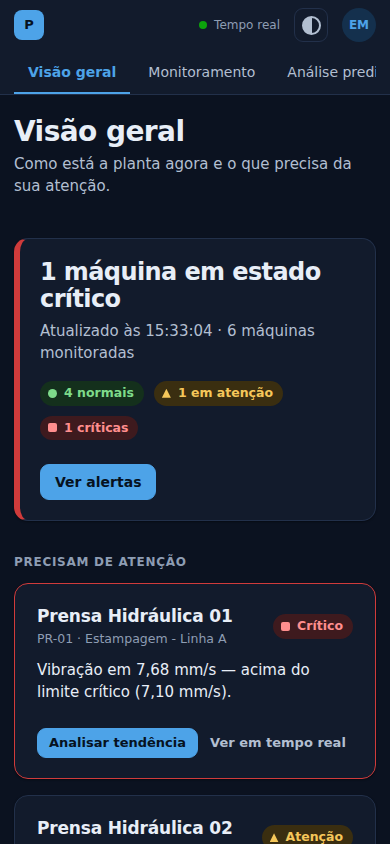
\includegraphics[height=0.45\textheight]{figuras/mobile.png}
\caption{Visão geral em tela de celular (390 px de largura).}\label{fig:mobile}
\end{figure}

\subsection{Cores e contraste}
\label{sec:cores}
A paleta usa o azul \texttt{\#00579D} como única cor de destaque (identidade, ações principais e séries dos gráficos), sobre neutros claros ou escuros. Cores
de estado (verde, âmbar, vermelho) são reservadas ao significado de estado e sempre acompanhadas de forma e texto. Cada gráfico mostra uma única série,
de modo que não há necessidade de paleta categórica. Os contrastes abaixo foram calculados pela fórmula de luminância relativa da WCAG:

\begin{table}[H]
\centering
\caption{Razões de contraste calculadas (mínimo: 4,5:1 para texto e 3:1 para elementos gráficos).}
\label{tab:contraste}
\small
\begin{tabular}{@{}l r r@{}}
\toprule
\textbf{Par (primeiro plano / fundo)} & \textbf{Tema claro} & \textbf{Tema escuro}\\
\midrule
Texto principal / superfície & 17,3 & 14,8\\
Texto secundário / superfície & 7,5 & 9,2\\
Texto terciário / superfície & 5,3 & 6,3\\
Azul de destaque / superfície & 7,4 & 6,3\\
Texto do botão primário / azul & 7,4 & 6,9\\
Chip ``normal'' (texto / fundo) & 5,9 & 8,4\\
Chip ``atenção'' (texto / fundo) & 6,3 & 8,4\\
Chip ``crítico'' (texto / fundo) & 6,6 & 6,9\\
Indicador verde / superfície & 3,4 & 5,1\\
Indicador vermelho / superfície & 4,8 & 3,6\\
Indicador âmbar / superfície & \textbf{1,8} & 9,4\\
\bottomrule
\end{tabular}
\end{table}

A única razão abaixo do mínimo é o indicador âmbar sobre fundo claro (1,8:1). Ela é compensada pela forma (triângulo) e pelo texto (``Atenção''), e as linhas
de limite no gráfico claro usam um âmbar mais escuro. O texto terciário no tema claro foi ajustado após a verificação (valor inicial reprovava sobre o
fundo da página).

% ------------------------------------------------------------------ 8
\section{Testes e verificação}
\label{sec:testes}
\subsection{Testes unitários}
Quatro testes (\codigo{pytest}) cobrem: limites de severidade bilaterais da pressão, monotonicidade do índice de saúde, \emph{debounce} do detector de alertas e a
estimativa de RUL em uma série linear conhecida (erro menor que 0,5 dia). Todos passam.

\subsection{Testes ponta a ponta}
Com o Chromium automatizado (Playwright) foram executados: conexão WebSocket (indicador ``Tempo real''), troca de variáveis e máquinas, injeção de falha,
notificação de novo alerta, reconhecimento do alerta, criação e andamento de ordem de serviço, alternância de tema e capturas de tela em desktop e celular.
Não foram escritos testes automatizados permanentes para a interface; esses roteiros foram executados durante o desenvolvimento.

\subsection{Defeitos encontrados e corrigidos}
\begin{itemize}
  \item A pasta \codigo{assets} não era carregada (o Dash a procurava dentro do pacote), deixando a página sem estilo. Corrigido apontando a pasta explicitamente.
  \item As faixas de limite não apareciam nos gráficos com subpainéis, pois o Plotly ignora formas em subpainéis vazios. Corrigido adicionando as séries antes das zonas.
  \item Alertas duplicados a cada reinício, porque o detector não conhecia condições já existentes. Corrigido inicializando o estado do detector e evitando
  duplicidade de alertas pendentes do mesmo problema.
  \item Erro 500 ao exibir a notificação de novo alerta (propriedade inválida num componente de link). Corrigido.
  \item Mensagem ``100,0 acima do limite de 100,0'' por arredondamento. Corrigida mostrando uma casa decimal adicional quando necessário.
\end{itemize}

\subsection{Medições de desempenho}
Valores medidos durante o desenvolvimento (máquina de desenvolvimento, servidor Flask local), na versão anterior ao redesenho final; devem ser remedidos
(a página \emph{Sobre} $\rightarrow$ \emph{Medições} refaz a medição em tempo real):

\begin{table}[H]
\centering
\caption{Medições de desempenho do protótipo.}
\label{tab:medicoes}
\begin{tabular}{@{}l r@{}}
\toprule
\textbf{Métrica} & \textbf{Valor}\\
\midrule
Histórico em CSV & 12\,096 linhas, 621 KB\\
Leitura do CSV (pandas, sem cache) & 10 ms\\
Cálculo de estado e índice de saúde (vetorizado) & 35 ms\\
Montagem de uma figura de telemetria (3 painéis, versão anterior) & 227 ms\\
Pacote do WebSocket por tick & 1,2 KB\\
Snapshot completo (equivalente a polling) & 28 KB\\
\bottomrule
\end{tabular}
\end{table}

O pacote por tick é cerca de 23 vezes menor que o snapshot completo, o que ilustra a vantagem do modelo \emph{push} sobre o \emph{polling}.

% ------------------------------------------------------------------ 9
\section{Diagnóstico crítico}
\label{sec:limitacoes}
Em atendimento à etapa de diagnóstico crítico da proposta, a equipe analisou o próprio protótipo.

\subsection{Falhas de usabilidade}
\begin{itemize}
  \item Não há filtro por turno ou linha; o usuário vê todas as máquinas, inclusive as que não são de sua responsabilidade.
  \item Limites são fixos no código; não podem ser ajustados por máquina na interface.
  \item O índice de saúde é uma métrica própria e precisa de explicação; há um bloco de detalhes na análise, mas faltam dicas contextuais nos cartões.
  \item Não existem perfis de usuário, autenticação nem trilha de auditoria nas ordens de serviço.
  \item A interface não foi validada com usuários reais; as decisões de design se baseiam em princípios e na avaliação da equipe.
\end{itemize}

\subsection{Gargalos de performance e arquitetura}
\begin{itemize}
  \item A cada tick, as figuras são reconstruídas no servidor; não escala para muitas máquinas e usuários simultâneos.
  \item CSV como banco: leitura completa a cada consulta e regravação integral de alertas e ordens; sem concorrência real entre processos.
  \item O estado do simulador fica na memória de um único processo; não funciona com vários \emph{workers}.
  \item O servidor de desenvolvimento do Flask é adequado à demonstração, não à produção.
  \item O RUL linear é impreciso quando a degradação não é linear ou a série é ruidosa; a confiança baixa é sinalizada, mas o modelo não foi validado com falhas reais.
\end{itemize}

\subsection{Oportunidades de melhoria}
\begin{itemize}
  \item Substituir o CSV por um banco de séries temporais (por exemplo, TimescaleDB ou InfluxDB) e ingerir sensores reais via MQTT ou OPC~UA.
  \item Atualizar o gráfico no navegador apenas com o ponto novo (\codigo{extendData}) e aplicar \emph{downsampling} em janelas longas.
  \item Modelos de degradação mais realistas (exponencial, filtro de Kalman) validados com dados reais.
  \item Servir com gunicorn e \emph{gevent}, com Redis \emph{pub/sub} para escalar o WebSocket.
  \item Perfis, autenticação, limites configuráveis e testes automatizados de interface.
\end{itemize}

% ------------------------------------------------------------------ 10
\section{Atendimento à rubrica}
\begin{table}[H]
\centering
\caption{Relação entre os critérios de avaliação e as evidências do projeto.}
\label{tab:rubrica}
\small
\begin{tabularx}{\textwidth}{@{}l r X@{}}
\toprule
\textbf{Critério} & \textbf{Peso} & \textbf{Evidência}\\
\midrule
Design e usabilidade & 20\% & Princípios da Gestalt e hierarquia aplicados (Seção~\ref{sec:design}); contrastes calculados (Tabela~\ref{tab:contraste}); estado por cor, forma e texto; uma pergunta por tela; revelação progressiva.\\
Programação e frameworks & 30\% & Dash/Plotly com callbacks reativos, gráficos interativos (hover, projeção, zonas), análises em Python e testes unitários (Seções~\ref{sec:framework} e 5).\\
Integração web & 20\% & WebSocket com reconexão, API REST, layout responsivo, tema claro/escuro, exportação CSV (Seção~\ref{sec:integracao}).\\
Postura crítica e argumentativa & 15\% & Comparativo de tecnologias, registro do redesenho, defeitos corrigidos e diagnóstico crítico (Seções~\ref{sec:fundamentacao}, 8 e 9).\\
Postura profissional e aprendizado & 15\% & Processo iterativo com revisão, incorporação de feedback e documentação (README e roteiro).\\
\bottomrule
\end{tabularx}
\end{table}

\paragraph{Entregáveis da proposta.} (1) Este relatório técnico; (2) repositório de código organizado em HTML/JS/Python; (3) aplicação web operacional para
demonstração em tempo real.

% ------------------------------------------------------------------ 11
\section{Conclusão}
O projeto entregou uma aplicação web operacional que cobre o tema específico (manutenção preditiva e telemetria de prensas, compressores e tornos) e os
tópicos gerais da proposta: fundamentos de UX, framework de código (Dash/Plotly), integração web (WebSocket e API REST) e uma discussão comparativa com ferramentas de BI.
O maior aprendizado de processo foi a necessidade de avaliar criticamente a primeira versão: reduzir a quantidade de informação, organizar a hierarquia e
orientar cada tela por uma pergunta do usuário tornou a interface mais clara do que a abordagem inicial de ``mostrar tudo''.

As limitações principais são o uso de dados simulados e limites fictícios, o CSV como banco, o redesenho das figuras no servidor e a ausência de validação com usuários reais.
Esses pontos foram documentados e orientam os próximos passos.

% ------------------------------------------------------------------ APÊNDICES
\appendix
\section{Como executar}
\begin{lstlisting}
pip install -r requirements.txt
python run.py            # http://localhost:8050
python -m predictive.datagen   # regenera os CSVs do zero
pytest                   # testes unitarios
\end{lstlisting}
Variáveis de ambiente opcionais: \codigo{PORT} (8050), \codigo{HOST} (127.0.0.1) e \codigo{TICK\_SECONDS} (2).

\section{Roteiro sugerido para a demonstração (15 minutos)}
\begin{enumerate}
  \item Visão geral (2 min): resumo, cartões de atenção, estado por cor, forma e texto.
  \item Monitoramento (2 min): abas de variável, zonas de limite, indicador de tempo real, tema escuro.
  \item Injeção de falha (2 min): modo demonstração, falha de rolamento na PR-01, notificação e estado crítico.
  \item Alertas (2 min): reconhecer, criar ordem, iniciar; ver \codigo{data/work\_orders.csv} mudar.
  \item Análise preditiva (3 min): PR-02, dias até o limite crítico, confiança e limitações.
  \item Argumentação (4 min): princípios de design, diagnóstico crítico, tecnologias e melhorias.
\end{enumerate}

% ------------------------------------------------------------------ REFERÊNCIAS
\begin{thebibliography}{99}
\bibitem{proposta} \textit{Trabalho de Pesquisa e Aplicação Prática: Engenharia e Design de Interfaces Analíticas na Indústria 4.0}. Proposta de trabalho (documento da disciplina).
\bibitem{few} FEW, S. \textit{Information Dashboard Design: The Effective Visual Communication of Data}. 2.\,ed. Analytics Press, 2013.
\bibitem{tufte} TUFTE, E. R. \textit{The Visual Display of Quantitative Information}. 2.\,ed. Graphics Press, 2001.
\bibitem{nielsen} NIELSEN, J. \textit{10 Usability Heuristics for User Interface Design}. Nielsen Norman Group, 1994.
\bibitem{wcag} W3C. \textit{Web Content Accessibility Guidelines (WCAG) 2.x}. World Wide Web Consortium.
\bibitem{rfc6455} FETTE, I.; MELNIKOV, A. \textit{The WebSocket Protocol}. RFC 6455, IETF, 2011.
\bibitem{iso20816} ISO 20816 (série). \textit{Mechanical vibration --- Measurement and evaluation of machine vibration}.
\bibitem{iso17359} ISO 17359. \textit{Condition monitoring and diagnostics of machines --- General guidelines}.
\bibitem{iso13374} ISO 13374 (série). \textit{Condition monitoring and diagnostics of machines --- Data processing, communication and presentation}.
\bibitem{dash} PLOTLY. \textit{Dash Documentation}. Disponível em: \url{https://dash.plotly.com}.
\bibitem{plotly} PLOTLY. \textit{Plotly Python Graphing Library}. Disponível em: \url{https://plotly.com/python/}.
\end{thebibliography}

\end{document}
